\documentclass[11pt,letterpaper]{article}

% PAQUETES ++++++++++++++++++++++++++++++++
\usepackage[utf8]{inputenc}
\usepackage[spanish]{babel}
\usepackage{amsmath}
\usepackage{amsfonts}
\usepackage{amssymb}
\usepackage[left=2cm,right=2cm,top=2cm,bottom=2cm]{geometry}
\pagenumbering{arabic}
\usepackage[pdftex]{graphicx}
\usepackage{tabularx}
\usepackage{tcolorbox}
\usepackage{array}
\usepackage{url}
\usepackage{relsize}
\usepackage{multirow}
\usepackage{float}
\usepackage{tabularray}
\tcbuselibrary{most}
\usepackage[dvipsnames]{xcolor}
\decimalpoint

%+++++++++++++++++++++++++++++++++++++++++++++++++++
\graphicspath{ {./img/}}
\pagenumbering{arabic}
\newtcolorbox{matlab-code}[2][]{colback=red!3!white, colframe=red!75!black, colbacktitle=red!75!black, enhanced, attach boxed title to top center={yshift=-2mm}, title={#2}, #1}



% +++++++++++++++++++++
\begin{document}
\title{Trabajo de Investigación: Ajuste de Curvas por Mínimos Cuadrados}

\author{
	Alberto Ramos Cruz
	\and Moisés Alonso Marroquín Ayala
	\and René Eduardo Hernández Castro
	\and Roberto José Melgares Zelaya
}
\maketitle


\section{Regresión lineal por mínimos cuadrados}
%++++++++++++++++++
%PUNTO 1 A ALBERTO
%+++++++++++++++++++++++++
\subsection{Ajuste de una recta por regresión por mínimos cuadrados}
Esta es una técnica que, dados un conjunto de pares ordenados $(X,Y)$, nos permite adaptar una recta que se acerque lo más posible a todos los puntos de manera que represente de mejor forma una serie de datos. De esta forma minimizando la suma de los cuadrados de las diferencias entre los valores observados $Y$ y los valores predichos por la recta, reduciendo así la diferencia entre los datos reales y la recta adaptada, para esto se necesita utilizar la fórmula general de una recta: $$ y = mx + b$$
Donde se tiene que: 
\begin{itemize}
	\item $y$ es el valor predicho por la fórmula como la variable dependiente.
	\item $x$ es el valor de la variable dependiente.
	\item $m$ es la pendiente de la recta.
	\item $b$ es la intersección de la recta con el eje $Y$.
\end{itemize}
Para este método lo que se busca encontrar es la pendiente $m$, por lo que recurrimos a la fórmula:
\begin{equation}
m = \frac{\sum_{i=1}^{n} x_iy_i - \frac{\sum_{i=1}^{n} x_i \sum_{i=1}^{n} y_i}{n}}{\sum_{i=1}^{n} x_i^2 - \frac{(\sum_{i=1}^{n} x_i)^2}{n}}
\end{equation}
Por otro lado, para encontrar $b$ hacemos uso de la fórmula:
\begin{equation}
b = \frac{\sum_{i=1}^{n} y_i - m\sum_{i=1}^{n} x_i}{n}
\end{equation}
Donde $n$ representa la cantidad de datos que se tienen en la serie de pares ordenados. De esta manera se garantiza, que la aproximación se acerque lo más posible a todos los puntos, minimizando el error cuadrático, y reflejando de manera más precisa la relación entre las variables.\cite{nieves2011metodos} \par A continuación, se demuestra un ejercicio resuelto haciendo uso del método anterior junto con un algoritmo en \textit{MATLAB}
\subsubsection*{\textcolor{Mahogany}{Problema asignado haciendo uso del método de ajuste de recta por mínimos cuadrados}}
\begin{center}
\textit{\textbf{Problema 1: } En la siguiente tabla, T es la temperatura de una bobina en °C  y r es la resistencia de la bobina en Ohms ($\Omega$). Ajuste una recta de mínimos cuadrados para representar r en términos de T. Estime cual sería la resistencia de una bobina que está a 65 °C. Posteriormente, grafique la recta de mínimos cuadrados y los puntos de la tabla en un solo plano cartesiano}.\linebreak \par
\begin{tabular}{c|cccccc}
 \hline 
 T (°C) & 10.50 & 29.49 & 42..70 & 60.01 & 75.51 & 91.05 \\ 
 \hline 
 r ($\Omega$) & 10.421 & 10.939 & 11.321 & 11.794 & 12.242 & 12.668 \\ 
 \hline 
 \end{tabular} 
\end{center}
Para este problema nuestra \textit{variable independiente} serán los valores de la temperatura \textit{T}, mientras que nuestra \textit{variable dependiente} serán los valores de la resistencia, por ello los valores de $X$ y $Y$ serán la temperatura y la resistencia, respectivamente. Comenzamos el algoritmo en \textit{MATLAB} agregando los datos iniciales y realizando las primeras sumas de los valores de $X$, $Y$,  $X^2$, y $XY$, sabiendo que $n = 6$. 

\begin{figure}[H]
\begin{tcolorbox}[title = Problema 1: Declaración de valores iniciales y sumatorias]
\begin{verbatim}
T = [10.50 29.49 42.70 60.01 75.51 91.05]; % X - variable independiente
R = [10.421 10.939 11.321 11.794 12.242 12.668]; % Y variable dependiente
n = length(T);

sumatoriaX = sum(T); % sumatoria de X
sumatoriaY = sum(R); % sumatoria de Y
multiXY=0; % Para la sumatoria de XY
X2=0; % Para la sumatoria de X^2

for i=1:n
    multiXY = multiXY+(T(i)*R(i));
    X2 = X2 + T(i)^2;
end
\end{verbatim}
\end{tcolorbox}
\end{figure}
Con los valores encontrados de las sumas, podemos pasar a  encontrar $m$ y $b$ para luego armar la función lineal de $r=mt + b$
\begin{figure}[H]
\begin{tcolorbox}[title = Problema 1: Armando la función lineal de aproximación]
\begin{verbatim}
% Obteniendo la pendiente en mi función y=mx+b que se reescribe como r = mT+b
m = (multiXY-((sumatoriaX*sumatoriaY)/n))/(X2-(sumatoriaX^2/n));

% Obteniendo el intersecto b de la función
b = (sumatoriaY-(m*sumatoriaX))/n;

%se escribe la función
syms t;
r = m*t+b;
\end{verbatim}
\end{tcolorbox}
\end{figure}

Con las líneas anteriores se obtienen finalmente los valores de la pendiente y el intercepto de la función lineal que se puede usar para aproximar valores. 
\begin{figure}[H]
\centering
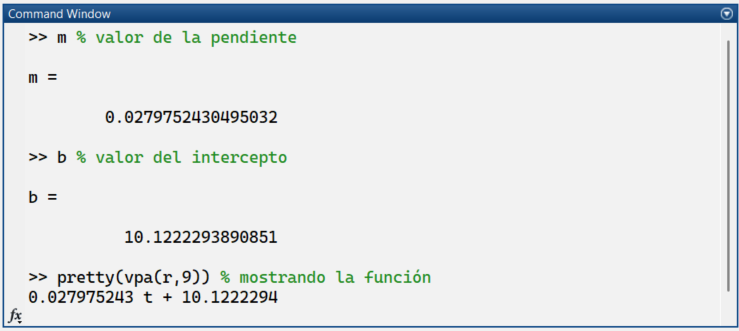
\includegraphics[width=4.5in]{eq1.png}
\caption{Los valores de $b$ y $m$ obtenidos con el algoritmo junto con la función}
\label{figure:lineal1} 
\end{figure}
Ahora es posible obtener la estimación deseada de la resistencia a una temperatura de 65 °C haciendo uso del comando \texttt{double(subs(r,65))}. Para finalizar el ejercicio, mostraremos cómo la gráfica de la recta se sobrepone a los valores iniciales provistos por el ejercicio. 
% resultado
\begin{figure}[H]
\centering
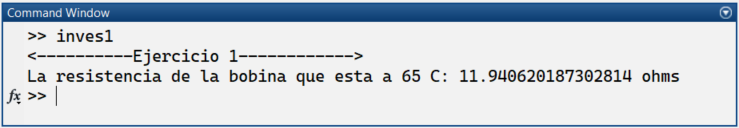
\includegraphics[width=4in]{res1.png}
\caption{Resultado de la evaluación de la función $r=mt + b$ en 65, obteniendo así una respuesta de \textbf{11.940620187302814 $\Omega$}}
\label{figure:res1}
\end{figure}
%grafica
\begin{figure}[H]
\centering
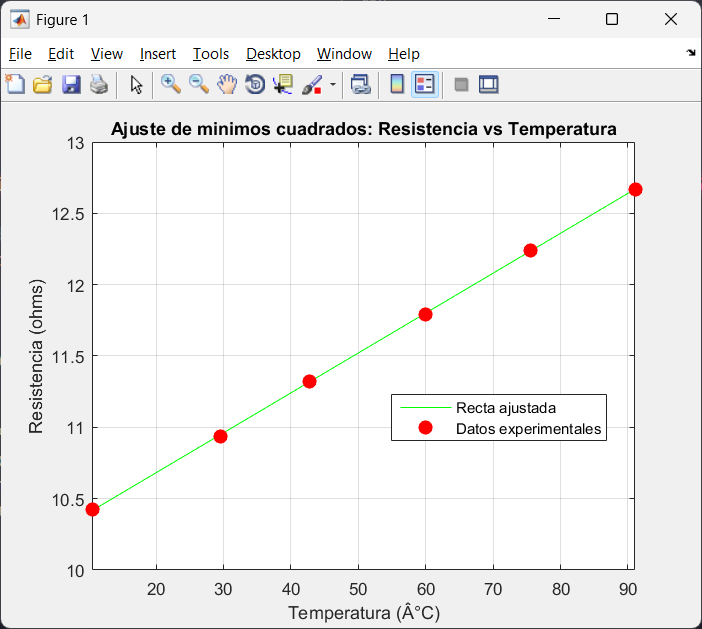
\includegraphics[width=3.5in]{recta.png}
\caption{Gráfica de la recta obtenida con el método de estudio con los valores iniciales de la temperatura y la resistencia sobre la misma. }
\label{figure:recta1}
\end{figure}

%---------------
%PUNTO 1 B // RENE
%---------------
\subsection{Linealización de relaciones no lineales}
Una función $y$ se puede formar mediante la combinación de múltiples funciones lineales $f_1$,$f_1$,\dots,$f_n$ y la minimización de la suma de los cuadrados de las diferencias entre la predicción del modelo y los datos generados en un sistema lineal de ecuaciones para los coeficientes del modelo. Si se construye de esta forma $y$ es lineal en sus coeficientes. En este caso analizaremos la posibilidad de convertir relaciones no lineales a su forma lineal de forma similar al método descrito anteriormente.\cite{ualberta} Consideraremos los siguientes modelos:
\begin{itemize}
	\item \textbf{Modelo Exponencial:} $y = \alpha e^{\beta x}$
	\item \textbf{Modelo Potencial:} $y = \alpha x^{\beta}$
\end{itemize}
\par Este tipo de modelos no lineales en $x$ y sus coeficientes desconocidos $\beta$ y $\alpha$ se pueden transformar en modelos lineales mediante el uso de logaritmo natural. Aplicando logaritmo natural a los modelos nos queda:
\begin{itemize}
	\item \textbf{Modelo Exponencial }($y = \alpha e^{\beta x}$) $\longrightarrow$ $\ln(y) = \beta x + \ln \alpha$
	\item \textbf{Modelo Potencial} ($y = \alpha x^{\beta}$) $\longrightarrow$ $\ln(y) = \beta \ln x + \ln \alpha$
\end{itemize}
\par 
En el caso del modelo exponencial se puede convertir como $(x_i, \ln(y_i))$ y con ello se puede hacer uso de la regresión lineal  para encontrar los coeficiente $\beta$ y $\alpha$. Para el caso del modelo potencial la información se puede expresar como $(\ln(x_i), \ln(y_i))$ y nuevamente hacer uso de la regresión lineal para encontrar los coeficientes $\beta$ y $\alpha$.\cite{ualberta}\cite{nieves2011metodos} 

\subsubsection{Modelo Exponencial}
Recordando la forma exponencial, $y = \alpha e^{\beta x}$, es posible linealizarla mediante el uso de logaritmo natural para obtener la forma $\beta x + \ln \alpha$ y convertir una serie de datos a $(x_i, \ln(y_i))$.  \cite{ualberta}
\par
Mediante el uso de regresión lineal es posible expresar $y^*$ como: \textbf{$y^* = \beta^* x + \alpha^*$ 	} obtendremos los coeficientes $\alpha^*$ y $\beta^*$ de la siguiente manera:

\begin{align} 
	\beta^* &= \frac{n \sum_{i=1}^{n} x_iy_i^* - \sum_{i=1}^{n} x_i \sum_{i=1}^{n} y_i^*}{n\sum_{i=1}^{n} x_i^2 - (\sum_{i=1}^{n}  x_i)^2} \label{equation:betaE}\\
	\alpha^* &= \frac{\sum_{i=1}^{n} y_i^* - \beta^* \sum_{i=1}^{n} x_i  }{n} \label{equation:alphaE}
\end{align}
%% EJEMPLO 1
\subsubsection*{\textcolor{Blue}{Ejemplo propuesto haciendo uso del modelo exponencial}}
\begin{center}
\textit{\textbf{Ejemplo 1:} Haremos un ajuste de modelo exponencial y potencial para la siguiente lista de datos: (1,1.93), (1.1,1.61), (1.2,2.27), (1.3,3.19), (1.4,3.19), (1.5,3.71), (1.6,4.29), (1.7,4.95), (1.8,6.07), (1.9,7.48), (2,8.72), (2.1,9.34), y (2.2,11.62).}
\end{center}
El procedimiento a continuación se realizará con los datos expresados para un caso de modelo exponencial, pero el procedimiento es el ``mismo'' para ambos modelos, cambiando únicamente su anotación final como veremos más adelante. Expresaremos los datos en formato de tabla para un mejor entendimiento, quedando de la siguiente manera. Se hará uso de $y*$ para representar $\ln(y_i)$\par
\begin{table}[H]
	\centering
	\begin{tabular}{c | c}
	\hline
		$x_i$ & $y_i$ \\ \hline
        1	& 0.6575 \\
        1.1	& 0.4762 \\
        1.2	& 0.8198 \\
        1.3	& 1.16 \\
        1.4	& 1.16 \\
        1.5	& 1.311 \\
        1.6	& 1.4563 \\
        1.7	& 1.5994 \\
        1.8	& 1.8034 \\
        1.9	& 2.0122 \\
        2	& 2.1656 \\
        2.1	& 2.2343 \\
        2.2	& 2.4527 \\ \hline
	\end{tabular}
\end{table}
Haciendo uso de la regresión lineal descrita anteriormente se obtendrán los valores de $\beta$ y $\alpha$. Los cuales serán
\begin{align*}
	\beta^* &= \frac{13 \times 33.8013 - 20.8\times19.3085}{13 \times 35.10 - (29.8)^2} = 1.5976 \\
	\alpha^* &= \frac{19.3085 - 1.5976 \times 20.8}{13} = -1.0709
\end{align*}
Con lo anterior ya obtenemos los valores para el modelo no lineal que necesitábamos de $\beta = \beta^* =  1.5976$, y $\alpha = e^{\alpha^*} = e^{-1.0709} = 0.3427$, haciendo posible armar la forma exponencial final como: $$y = 0.3427e^{1.5976x}$$

\subsubsection*{\textcolor{Mahogany}{Problema asignado haciendo uso del modelo potencial}}
\begin{center}
	\textit{\textbf{Problema 2: }Para calibrar un medidor de orificio, se miden la velocidad $v$ de un fluido y la caída de presión $\Delta P$. Los datos experimentales se dan a continuación y se buscan los mejores parámetros $a$ y $b$ de la ecuación que represente estos datos:}
	$$v= a (\Delta P)^b$$
	\textit{Donde:}
		\par $v =$ \textit{ velocidad promedio (pies/s) }\par $\Delta P =$\textit{caída de presión (mm Hg)}\linebreak \par
	\begin{tabular}{l|ccccccccccc}
		\hline 
		$i$ & 1 & 2 & 3 & 4 & 5 & 6 & 7 & 8 & 9 & 10 & 11 \\ 
		\hline 
		$v_i$ & 3.83 & 4.17 & 4.97 & 6.06 & 6.71 & 7.71 & 7.51 & 7.98 & 8.67 & 9.39 & 9.89 \\ 
		\hline 
		$\Delta P_i$ & 30 & 35.5 & 50.5 & 75 & 92 & 105 & 115 & 130 & 153.5 & 180 & 199.5 \\ 
		\hline 
	\end{tabular} 
	\linebreak\par
	\textit{Use la función encontrada para estimar la velocidad del fluido para una caída de presión de 5.5 mmHg. Grafique la función y los puntos de la tabla en un solo plano cartesiano.}
\end{center}
Con este problema, comenzaremos declarando los valores de la diferencia de presión y la velocidad promedio en \textit{MATLAB}. Debido a la forma de la ecuación de la velocidad promedio, haremos uso del \textbf{modelo potencial}, con el cual buscaremos encontrar los valores de $a$ y $b$.
\begin{figure}[H]
\begin{tcolorbox}[title = Problema 2: Valores y sumas iniciales para linealización]
\begin{verbatim}
% Valores de la Diferencia de Presión y Velocidad Promedio
DP = [30.0 35.5 50.5 75.0 92.0 105.0 115.0 130.0 153.5 180.0 199.5];
V =[3.83 4.17 4.97 6.06 6.71 7.17 7.51 7.98 8.67 9.39 9.89];
f = log(x);
val = 5.5; % valor al que queremos aproximar
%Calculamos las xi y yi
xi_lndp = double(subs(f,DP));
yi_lnv = double(subs(f,V));
n= length(DP);
  for i=1:n % Ciclo para calcular las sumas
    %Calculamos las xi*yi
    xiyi(i)= xi_lndp(i)*yi_lnv(i);
    %Calculamos las xi^2
    xi2(i) = (xi_lndp(i))^2;
  end
%Calculamos las sumatorias
sum_xiyi = sum(xiyi);
sum_xi =sum(xi_lndp);
sum_yi =sum(yi_lnv);
sum_xi2 =sum(xi2);
\end{verbatim}
\end{tcolorbox}
\end{figure}

Ahora que hemos calculado los valores de las sumas necesarias, podemos pasar a obtener los valores de $a$ y $b$ haciendo uso de las ecuaciones \textbf{\ref{equation:alphaE}} y \textbf{\ref{equation:betaE}}, donde $\alpha$ y $\beta$ corresponden a $a$ y $b$, respectivamente. Una vez hemos encontrado dichos valores, pasaremos a armar el modelo potencial del problema y aproximar al valor deseado.

\begin{figure}[H]
\begin{tcolorbox}[title = Problema 2: Calculando los valores de a y b]
\begin{verbatim}
%Calculamos b y a
b = ((n)*(sum_xiyi)-(sum_xi)*(sum_yi))/((n)*(sum_xi2)-(sum_xi)^2);
a = ((sum_yi)-(b)*(sum_xi))/(n);

alpha= exp(a); 	betha = b;

% ARMANDO EL MODELO POTENCIAL
modelo = alpha * (x ^ (betha));
\end{verbatim}
\end{tcolorbox}
\end{figure}
%%Imagens de resultados ejercicio 2
\begin{figure}[H]
\centering
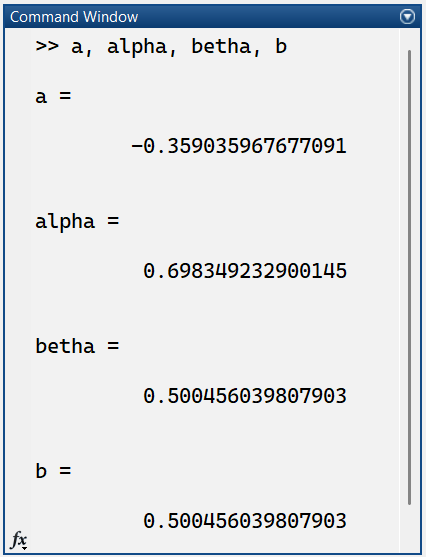
\includegraphics[width=2.5in]{ab2.png}
\caption{Valores obtenidos de a, b, $\alpha$ y $\beta$ para este ejercicio con una precisión de 15 decimales}
\label{figure:ab2}
\end{figure}

\begin{figure}[H]
\centering
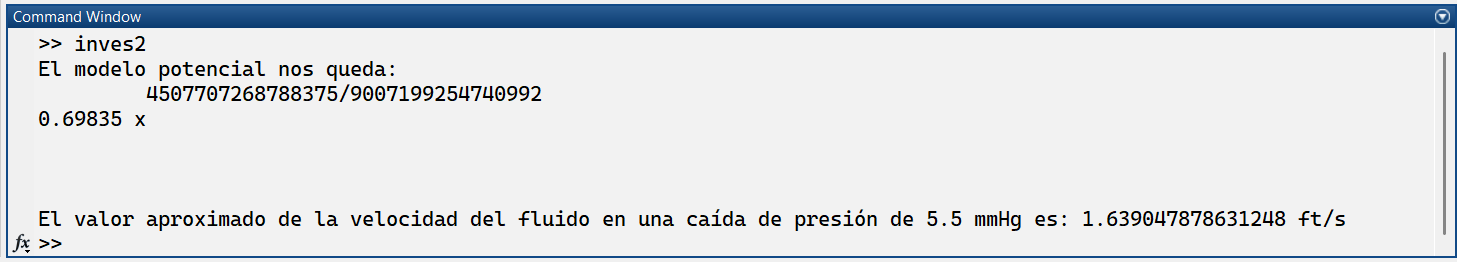
\includegraphics[width=5in]{res2.png}
\caption{Función obtenida que describe la aproximación de la función junto con la aproximación del valor buscado por medio de extrapolación, pues el valor al que queremos aproximar está fuera del intervalo de los datos dados para $\Delta P$.}
\label{figure:res2}
\end{figure}
Ya que hemos obtenido el modelo, y la aproximación en el valor que buscabamos, podemos pasar a la gráfica de la función.
\begin{figure}[H]
\centering
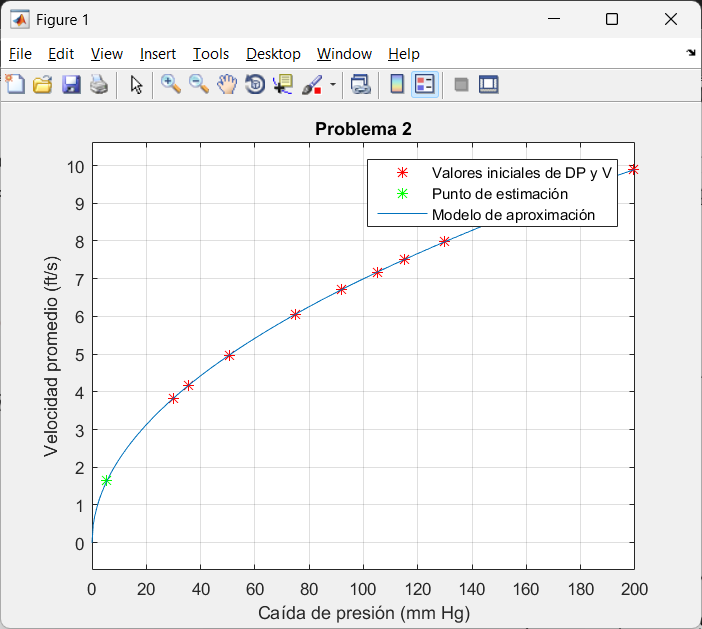
\includegraphics[width=2.7in]{graf2.png}
\caption{Gráfica del modelo potencial encontrado, junto con los puntos de los valores iniciales y el valor inicial sobrepuestos sobre esta.}
\label{figure:graf2}
\end{figure}
% AAAAAAAAAAAAAAAAAAAAAAAA METODO POTENCIAL
\subsubsection{Modelo Potencial}
El modelo potencial, como vimos anteriormente, viene dado por la forma $y = \alpha x^{\beta}$. Para el método potencial, es necesario sustituir los valores $x_i$ en la \textbf{Ecuación \ref{equation:betaE} } y la \textbf{Ecuación \ref{equation:alphaE}} por las $x^*$ que corresponden a la evaluación de $\ln(x_i)$. \par En el caso de la linealización del modelo potencial, recordando su forma $y = \alpha e^{\beta x}$, también se debe de linealizar haciendo uso de logaritmo natural obteniendo $\beta \ln x + \ln \alpha$ , con ello convertiremos los datos a la forma final $(\ln(x_i), \ln(y_i))$. 

\subsubsection*{\textcolor{Mahogany}{Problema asignado haciendo uso del modelo potencial}}
\begin{center}
\textit{\textbf{Problema 3:} Ajuste los datos siguientes con el modelo potencial ($y = \alpha x^\beta$). Use la ecuación encontrada para hacer el pronóstico de $x$ en $x=9$. Represente gráficamente la función de aproximación junto con los datos.}
\linebreak\par
\begin{tabular}{c|cccccccccc}
\hline 
$x$ & 2.5 & 3.5 & 5 & 6 & 7.5 & 10 & 12.5 & 15 & 17.5 & 20 \\ 
\hline 
$y$ & 13 & 11 & 8.5 & 8.2 & 7 & 6.2 & 5.2 & 4.8 & 4.6 & 4.3 \\ 
\hline 
\end{tabular} 
\end{center}
De la misma forma que hemos resuelto los problemas anteriores, este problema también será resuelto por medio de un algoritmo en \textit{MATLAB}.
\begin{figure}[H]
\begin{tcolorbox}[title = Problema 3: Valores y sumas iniciales para linealización]
\begin{verbatim}
syms x;
X = [2.5 3.5 5 6 7.5 10 12.5 15 17.5 20];
Y = [13 11 8.5 8.2 7 6.2 5.2 4.8 4.6 4.3];
val = 9; % valor al que haremos la estimación

%Calculamos las xi y yi
f = log(x); % funcion logaritmo natural
xi_lnx = double(subs(f,X));
yi_lny = double(subs(f,Y));
n= length(X);

for i=1:n
    %Calculamos las xi*yi
    xiyi(i)= xi_lnx(i)*yi_lny(i);
    %Calculamos las xi^2
    xi2(i) = (xi_lnx(i))^2;
end

%Calculamos las sumatorias
sum_xiyi = sum(xiyi); % sumatoria de xy
sum_xi =sum(xi_lnx); % sumatoria de xi
sum_yi =sum(yi_lny); % sumatoria yi
sum_xi2 =sum(xi2); % sumatoria xi^2
\end{verbatim}
\end{tcolorbox}
\end{figure}
Una vez hemos obtenido los valores de las sumatorias $\Sigma x$, $\Sigma xy$, $\Sigma x^2$, y $\Sigma y$ podemos pasar a calcular los valores de los coeficientes $\beta$ y $\alpha$. Posteriormente, armaremos la función final para la aproximación.
\begin{figure}[H]
\begin{tcolorbox}[title = Problema 3: Obteniendo los coeficientes y la función de aproximación]
\begin{verbatim}
%Calculamos b y a
b = ((n)*(sum_xiyi) - (sum_xi) * (sum_yi))/((n)*(sum_xi2)-(sum_xi)^2);
a = ((sum_yi)-(b) * (sum_xi))/(n);
alpha= exp(a); beta = b;

%Nuestra funcion nos queda como:
modelo = alpha*(x^(beta));
pretty(vpa(modelo, 5))
\end{verbatim}
\end{tcolorbox}
\end{figure}
\begin{figure}[H]
\centering
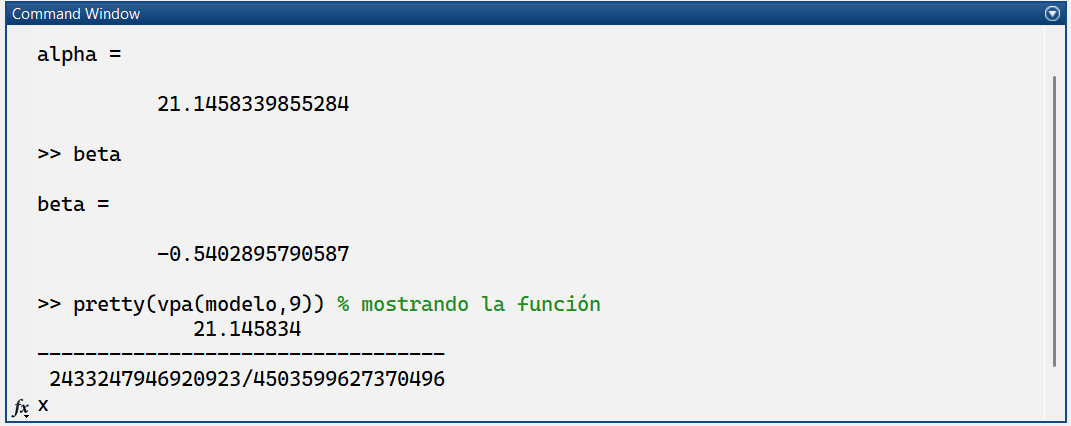
\includegraphics[width=4in]{ab3.png}
\caption{Los valores de $\alpha$ y $\beta$ encontrados. Abajo se muestra el modelo encontrado con los coeficientes en \textit{MATLAB}}
\label{figure:ab3}
\end{figure}
Ahora que hemos encontrado el modelo que describe la función, podemos representarlo de forma gráfica en un plano cartesiano con los valores iniciales dados sobre el modelo. También mostraremos la respuesta, la cual es la evaluación del valor a aproximar en el modelo encontrado.
\begin{figure}[H]
\centering
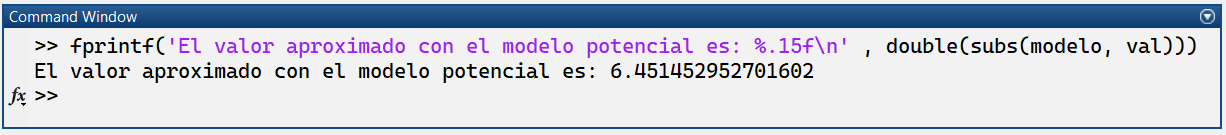
\includegraphics[width=6in]{res3.png}
\caption{Resultado de la evaluación del modelo en $x=9$, con esto obtenemos que la respuesta es: \textbf{6.451452952701602}}
\label{figure:res3}
\end{figure}
\begin{figure}[H]
\centering
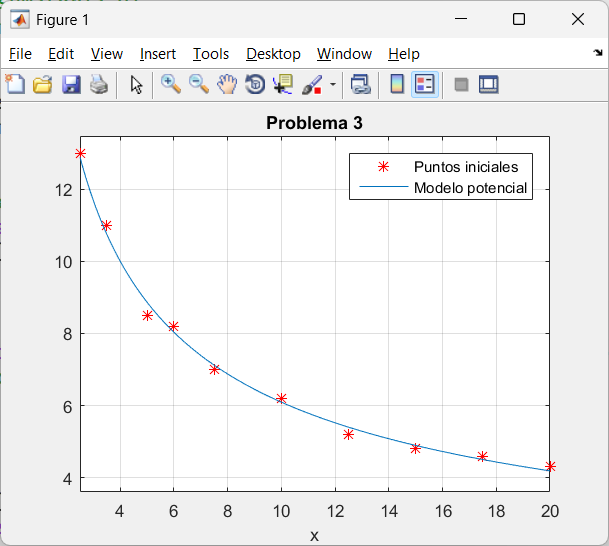
\includegraphics[width=2.8in]{exp3.png}
\caption{Gráfica del modelo con los puntos iniciales sobrepuestos en un plano cartesiano.}
\label{figure:graf3}
\end{figure}


%% PARA CALCULAR ERROR
\subsubsection{Coeficiente de determinación para relaciones no lineales}
Para determinar qué tanto los datos se ajustan al modelo se hará uso del ``coeficiente de determinación'', si bien este coeficiente puede variar dependiendo de que herramienta de software o artículo se ha obtenido, en nuestro caso haremos uso de lo siguiente:
\begin{equation}\label{equation:coeficiente}
	R^2 = 1 - \frac{\sum_{i=1}^{n} (y_i - y(x_i ) ^2 }
	{\sum_{i=1}^{n} (y_i)^2}
\end{equation}

Donde $R^2$ es equivalente a 1 menos el coeficiente entre la suma de cuadrados del modelo y la suma total de cuadrados de los datos. Esta definición de $R^2$ es la mas común usada para modelos no lineales.

%Ejemplo RENE

%---------------
%PUNTO 2
%---------------
\section{Aproximación polinomial con mínimos cuadrados}
Con el fin de encontrar un modelo matemático que represente lo mejor posible a una serie de datos experimentales, es posible abordarlo por medio de una curva $y=\phi(x)$ que se aproxime a los datos, sin la necesidad de que esta curva pase por ellos.
Lo anterior plantea el problema de verificar que en los términos:
$\{(x_i, y_i)\quad i = 0,1,2,3, \cdots, N\} $ se debe de hallar un $\phi(x)$ que verifique
\begin{equation}\label{equation:minima}
Minima = \sum_{i=0}^{N} (y_i - \phi(x_i))^2
\end{equation}


Para evitar problemas de derivabilidad se suele utilizar una diferencia cuadrada. \cite{binomiosScribd}
\subsection{Parábola de mínimos cuadrados}
La parábola de mínimos cuadrados tiene como objetivo aproximar un conjunto de puntos 
$(x_0, y_0),$ $(x_1, y_1),$ $ (x_2, y_2),$ $ \cdots , (x_N, y_N)$, donde $N$ es el número de elementos en el conjunto de puntos, 
a través de una curva polinomial de grado 2. Entonces, podemos entender la parábola de mínimos cuadrados como una curva de $y=\phi(x)$ donde $\phi(x)$ es un polinomio de segundo grado que viene dado por la ecuación
\begin{equation}\label{equation:parab-eq}
y = a_0 + a_1 x + a_2 x^2  
\end{equation}

donde $a_0, a_1, a_2 \in R$ y se determinan resolviendo las ecuaciones simultaneas : 

\begin{equation} \label{eq:sist-parab} 
	\left\{
		\begin{array}{@{}l@{}}
			\sum_{i=0}^{N} y_i  = a_0N + a_1\sum_{i=0}^{N} x_i + a_2\sum_{i=0}^{N} x_i^2 \cr\cr
			\sum_{i=0}^{N} x_iy = a_0\sum_{i=0}^{N} x_i + a_1\sum_{i=0}^{N} x_i^2 + a_2\sum_{i=0}^{N} x_i^3 \cr\cr
			\sum_{i=0}^{N} x_i^2y = a_0\sum_{i=0}^{N} x_i^2 + a_1\sum_{i=0}^{N} x_i^3 + a_2\sum_{i=0}^{N} x_i^4 		
		\end{array}
	\right.
\end{equation}
\linebreak 
Las ecuaciones anteriores  son conocidads como \textit{ecuaciones normales de mínimos cuadrados}. Estas ecuaciones se obtienen al multiplicar la ecuación $y = a_0 + a_1 x + a_2 x^2  $ por  1, $x$, y $x^2$, respectivamente. Como se puede observar, se obtiene un \emph{sistema con 3 incógnitas y 3 ecuaciones.}
\par
Para obtener los valores que acompañan a las incógnitas $a_i$ en el sistema de ecuaciones se debe de obtener la suma de los productos, tomando en cuenta los valores respectivos de $x_i$ con sus imágenes en $y_i$; esto a excepción del valor $N$ que acompaña a la incógnita $a_0$ en la primera ecuación como se puede observar en la Ecuación \ref{eq:sist-parab}.
\par
A continuación, se procede a resolver el sistema de ecuaciones por medio de una matriz de 4$\times$3 para que de este modo se obtengan los valores de las 3 incógnitas. \cite{spiegel}\cite{nieves2011metodos} En este caso, se puede usar cualquier método de resolución de sistemas de ecuaciones por medio de matrices, aunque para esta investigación se hará uso del método de Cramer. \emph{ Con el objetivo de mejorar la comprensión lectora, a partir de este punto se usará la siguiente notación.}

 \begin{table}[H]
 \centering
	\begin{tabular}{ c | c }
	\hline
	Símbolo & Significado  \\ \hline
	$X$ &	$\mathlarger{\Sigma} x_i$  \\ 
	$Y$ &   $\mathlarger{\Sigma} y_i$ \\
	$X^2$ & $\mathlarger{\Sigma} x_i^2$ \\
	$X^3$ & $\mathlarger{\Sigma }x_i^3$ \\ 
	$X^4$ & $\mathlarger{\Sigma} x_i^4$ \\
	$XY$ &  $\mathlarger{\Sigma} x_i y_i$	\\
	$X^2Y$& $\mathlarger{\Sigma} x^2_i y_i$	\\ \hline
	\end{tabular}
	\label{table:simbologia}
\end{table}

Usando la notación anterior, pasamos a resolver la matriz y obtener las ecuaciones que nos dan los determinantes. \emph{Recordar que estas matrices no contienen variables simbólicas, sino que valores escalares representados con letras mayúsculas.}
\begin{table}[H] \centering \begin{tabular}{c c c c c}
%% resolucion a0
$a_0 = \frac{
		\begin{vmatrix}
		 	Y &	X	& X^2 \\
		 	XY &	X^2	& X^3 \\
		 	X^2Y & X^3 & X^4	 
		\end{vmatrix}}
		{\begin{vmatrix}
		 	N &	X	& X^2 \\
		 	X &	X^2	& X^3 \\
		 	X^2 & X^3 & X^4	 
		\end{vmatrix}}
		
$ & &
% resolucion a1
$ a_1 = \frac{
		\begin{vmatrix}
		 	N &	Y	& X^2 \\
		 	X &	XY	& X^3 \\
		 	X^2 & X^2Y & X^4 
		\end{vmatrix}}
		{\begin{vmatrix}
		 	N &	X	& X^2 \\
		 	X &	X^2	& X^3 \\
		 	X^2 & X^3 & X^4	 
		\end{vmatrix}}
$ & &
% resolucion a2
$ a_2 = \frac{
		\begin{vmatrix}
		 	N &	X	& Y \\
		 	X &	X^2	& XY \\
		 	X^2 & X^3 & X^2Y 
		\end{vmatrix}}
		{\begin{vmatrix}
		 	N &	X	& X^2 \\
		 	X &	X^2	& X^3 \\
		 	X^2 & X^3 & X^4	 
		\end{vmatrix}}
$ \\
\end{tabular} \end{table}
%% PROBLEMA 4
\subsubsection*{\textcolor{Mahogany}{Problema asignado usando el método de la parábola de mínimos cuadrados}}
\begin{center}
	\textit{\textbf{Problema 4:} En la investigación de accidentes automovilísticos, el tiempo total requerido para el frenado total de un automóvil después de que el conductor ha percibido un peligro está compuesto de su tiempo de reacción (el tiempo que transcurre en su detección del peligro y la aplicación de los frenos) más el tiempo de frenado (el tiempo que tarda el automóvil en detenerse después de la aplicación de los frenos). La siguiente tabla proporciona la distancia de frenado D en metros de un automóvil que viaja a diversas velocidades V en metros por segundo al momento en el cual el conductor detecta un peligro.}
	\linebreak\par
	\begin{tabular}{c| c c c c c c }
	\hline
		Velociad V(m/s) &   20 & 30 & 40 & 50 & 60 & 70 \\ 		\hline
		Distancia de frenado D(m) & 54 & 90 & 138 & 206 & 292 & 396 \\
		\hline
	\end{tabular}
	\begin{itemize}
		\item \textbf{a)} Encontrar la ecuación de la parábola de mínimos cuadrados que ajuste esta serie de datos.
		\item \textbf{b)} Estimar la distancia $D$ de frenado cuando el automóvil se esta desplazando a 55 m/s y a 75 m/s.
		\item \textbf{c)} Grafique la paráboa y los puntos de la tabla en un mismo plano cartesiano.
	\end{itemize}
\end{center}

Para resolver este problema haremos uso de \emph{MATLAB} de la siguiente forma. En este caso las $X$ las usaremos como los valores $V$ de velocidad, mientras que los valores de $Y$ serán la distancia $D$
%Implementacion matlab1
\begin{figure}[H]
\begin{tcolorbox}[title=Problema 4: Implementación en MATLAB]
	\begin{verbatim}
		%% Declarando los arreglos de los valores
		X = [20, 30, 40, 50, 60, 70]
		Y = [54, 90, 138, 206, 292, 396]
		suma_X = 0; suma_X2 = 0;
		suma_X3 = 0; suma_X4 = 0;
		suma_Y = 0; suma_XY = 0;
		suma_X2Y = 0;
		N = length(X); % Tamaño de la matriz de X
		% Sumas de cada uno de los valores que se usaran para armar la matriz 
for i = 1: N
    suma_X = suma_X + X(i); % Suma Xi
    suma_X2 = suma_X2 + X(i) ^ 2; % Suma Xi^2
    suma_X3 = suma_X3 + X(i) ^ 3; % Suma Xi^3
    suma_X4 = suma_X4 + X(i) ^ 4; % Suma Xi^4
    suma_Y = suma_Y + Y(i); % Suma Yi
    suma_XY = suma_XY + X(i) * Y(i); % Suma Xi * Yi
    suma_X2Y = suma_X2Y + X(i) ^ 2 * Y(i); % Suma Xi^2 * Yi
end
\end{verbatim}
\end{tcolorbox}
\end{figure}
Con esto podemos armar la matriz  \texttt{M} , y la submatriz \texttt{subM}, que contendrán la matriz principal con los datos de las sumas de X, y los valores de los resultados respectivamente. A su vez, haremos uso de una matriz auxiliar \texttt{Maux} que será una copia de la matriz original, con los valores de la submatriz \texttt{subM} en una de las columnas como lo requiere el método de determinantes.
%matlab3
\begin{figure}[H]
\begin{tcolorbox}[ title=Problema 4: Implementación en MATLAB]
		\begin{verbatim}
		%% Creacion de la matriz M y submatriz subM
M = [ N suma_X suma_X2; suma_X suma_X2 suma_X3; suma_X2 suma_X3 suma_X4];
subM = [suma_Y suma_XY suma_X2Y];

%% encontrando los valores de a0, a1 y a2.
for i = 1:3
    Maux = M; %matriz auxiliar copia la original
    Maux(:,i) = subM; % reemplaza los valores de la columna
    a(i) = det(Maux) / det(M); % denominador del auxiliar con el de la original
end
\end{verbatim}
\end{tcolorbox}
\end{figure}
\begin{figure}[H]
\centering
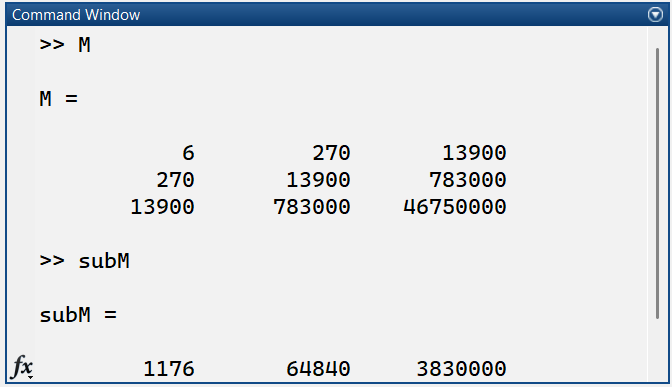
\includegraphics[width=2.8in]{mtz4.png}
\caption{Matriz obtenida con los valores del sistema de ecuaciones. Abajo, la submatriz de resultados del mismo sistema}
\label{figure:mtz4}
\end{figure}
La demostración anterior queda resuelta la matriz y obtenemos los valores de $a_n$ (es de notar al lector que \textit{MATLAB} cuenta los arreglos y matrices desde el 1 por lo que \texttt{a(1)} es igual a $a_0$ los cuales son: \par. 
\begin{align}
a_0 &= 41.771428571430754 \\
a_1 &= -1.095714285714397 \\
a_2 &= 0.087857142857144 \label{equation:aParab}
\end{align}
Con la matriz resuelta, junto con el arreglo con los valores de $a_0$, $a_1$ y $a_2$ podemos armar el polinomio en \textit{MATLAB} para resolver los incisos \textbf{a)} y \textbf{b)} evaluando la ecuación en los valores asignados. Por lo cual la ecuación de parábola que aproxima los datos es: 
$$P^2(x) =  41.771428571430754  - 1.095714285714397x + 0.087857142857144x^2$$ 

\begin{figure}[H]
\begin{tcolorbox}[title=Problema 4: Implementación en MATLAB]
\begin{verbatim}
syms x;
P = a(1) + a(2) * x  + a(3) * x ^ 2;
aprox = subs(P, v); % v es el valor de la velocidad al que deseamos aproximar
\end{verbatim}
\end{tcolorbox}
\end{figure}
Ahora que tenemos evaluado el polinomio que describe la parábola, podemos evaluarlo en los valores para $x=55$ y $x=75$ para obtener una aproximación de la distancia requerida a esas velocidades, propuestas por el literal \textbf{b)}. Por lo tanto obtenemos las siguientes evaluaciones en el polinomio \texttt{P} en \textit{MATLAB}:
\begin{figure}[H]
\centering
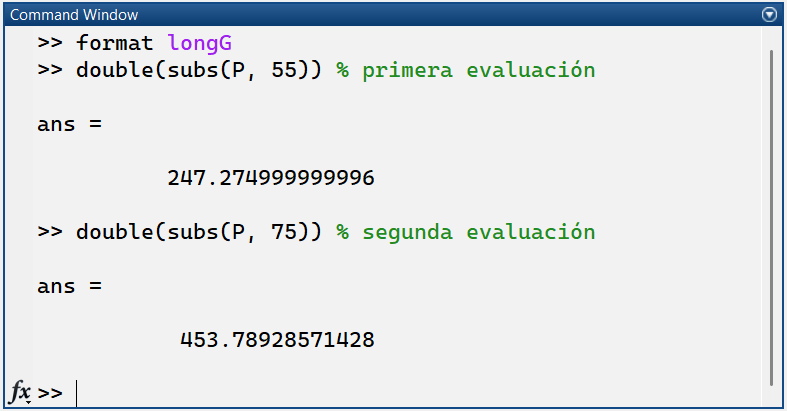
\includegraphics[width=3.5in]{res4.png}
\caption{Evaluaciones del polinomio de grado dos para $x=55$ y $x=75$.}
\label{figure:res4}
\end{figure}
A continuación se muestra como los valores iniciales como se indica en el literal \textbf{c)} se ven sobre la parábola creada. Donde se muestran los valores iniciales sobre la parábola construida:
\begin{figure}[H]
\centering
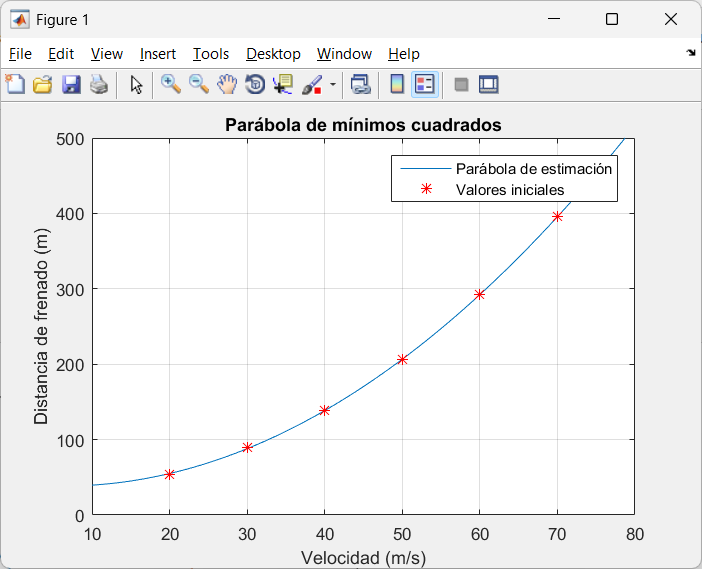
\includegraphics[width=3in]{parab4.png}
\caption{Gráfica de la parábola de estimación resultando con los valores iniciales sobrepuestos en un mismo plano cartesiano.}
\label{figure:parab4}
\end{figure}

% ++++++++++++++++++++++++
% SECCION 2B
%++++++++++++++++++++++++
\subsection{Ajuste de polinomios de grado \textit{n}	 (caso general)}
Si se desea aproximar una función dada de la forma tabular (pares x, y), de un polinomio grado N se realiza un procedimiento bastante similar al caso de la parábola de mínimos cuadrados. Para esto se debe minimizar la siguiente función:
\begin{equation} \label{	equation:ajuste}
	\sum_{i=1}^{m} \quad [ a_0 + a_1x_i + a_2x_i^2 + \dots + a_nx_i^n - f(x_i)] ^ 2
\end{equation}
\par
Para minimizar la función se debe derivar parcialmente con respecto a cada coeficiente $a_i$ desde 0 hasta $n$, para luego igualar a cero cada una de las funciones que se obtengan. De esta forma se llegará al siguiente sistema de ecuaciones lineales.
\begin{align}\label{equation:sist-gradon}
	ma_0 + a_1\Sigma x + a_2\Sigma x^2 + \dots + a_n\Sigma x^n &= \Sigma y \\
	a_0\Sigma x + a_1\Sigma x^2 + a_2\Sigma x^3 + \dots + a_n\Sigma x^{n+1} &= \Sigma xy\\
	a_0\Sigma x ^2 + a_1\Sigma x^3 + a_2\Sigma x^4 + \dots + a_n\Sigma x^{n+2} &= \Sigma x^2y \\
	\dots  & \dots \\
	a_0\Sigma x^n + a_1\Sigma x^{n+1} + a_2\Sigma x^{n+2} + \dots + a_n\Sigma x^{2n} &= \Sigma  x^ny
\end{align}
\par
Una vez obtenido este sistema de ecuaciones se puede resolver mediante matrices o cualquier otro método de resolución de sistemas de ecuaciones.
\par  Una vez encontrados los valores de todos los coeficientes se puede crear el polinomio de la forma  $p(n) = a_0 + a_1x + a_2x^2 + a_3x^3 + \dots + a_nx^n$ . Este es una expansión del método anterior que se desarrolló, puesto que a partir de esta forma general se puede obtener el caso de la parábola cuando se trabaja con un polinomio de grado $n = 2$.\cite{nieves2011metodos} 
\subsubsection{Error de aproximación del método}
Encontrar un polinomio de aproximación que pase por los puntos dados en forma tabular a veces tiene errores significativos; por ejemplo, cuando proviene de medidas físicas. En estas circunstancias no tiene sentido pasar un polinomio de aproximación por los puntos dados, sino sólo cerca de ellos.\par
No obstante, esto crea un problema, ya que se puede pasar un número infinito de curvas entre los puntos. Para determinar la mejor curva se establece un criterio que la fije y una metodología que la determine. \cite{binomiosScribd} El criterio más común consiste en pedir que la suma de las distancias calculadas entre el valor de la función que aproxima $p(x)$ y el valor de la función $f(x)$ dada en la tabla, sea mínima (ver \textbf{ecuación \ref{equation:minima}}), es decir, que:

\begin{equation}\label{equation:minimo}
\sum_{i=1}^m | p(x_i) - f(x_i) | = \sum_{i=1}^m d_i = minimo
\end{equation}

\par
A continuación, se muestra un ejemplo práctico para su comprensión junto con un algoritmo de resolución en \textit{MATLAB}.

%% Ejemplo
\subsubsection*{\textcolor{Blue}{Ejemplo propuesto haciendo uso del método de ajusto de polinomios usando $n=4$}}
\begin{center}
\textit{\textbf{Ejemplo 2:} El calor específico $C_p$ (cal/kg mol) del $Mn_3O_4$ varía con la temperatura. A partir de la siguiente tabla, aproxime la información con un polinomio por el método de mínimos cuadrados.} \cite{nieves2011metodos}
\linebreak \par
	\begin{tabular}{c|c c c c c c}
	\hline 
	T (°K) & 280 & 650 & 1000 & 1200 & 1500 & 1700 \\ \hline
	$C_p$ (cal/kg mol) & 32.7 & 45.4 & 52.15 & 53.7 & 52.9 & 50.3 \\ 
	\hline 
	\end{tabular} 
\end{center}

Se hará uso del siguiente algoritmo en \textit{MATLAB} para mostrar el resultado de este método con $n=4$
\begin{figure}[H]
\begin{tcolorbox}[title=Ejemplo 2: Implementación en MATLAB]
\begin{verbatim}
syms x;
X = [280 650 1000 1200 1500 1700];
Y = [32.7 45.4 52.15 53.7 52.9 50.3];
xEvaluar = 1500;
%n se ocupará para indicar el grado del polinomio
n = 4;
% Guardar el valor de la sumatoria de Y
sumY = sum(Y);
%Guardar en un vector las sumas de todos los valores de X elevadas a sus
%potencias desde 1 hasta 2n 
for i=1:2*n
    sum = 0;
   for j=1:length(X)
       sum = sum + (X(j))^i;
   end
   sumXs(i) = sum;
end
%Creando un vector que almacene los resultados de la matriz
for i=1: n+1
    if i == 1
        resM(i) = sumY; 
    else
        sumatoria = 0;
        for j=1:length(X)
             sumatoria = sumatoria + Y(j)*X(j)^(i-1);
        end
        resM(i) = sumatoria;
    end
end
\end{verbatim}
\end{tcolorbox}
\end{figure}
El algoritmo anterior nos ayuda a dar las sumas de los valores requeridos, los cuales son almacenados dentro de una matriz \texttt{sisM} como veremos a continuación donde se llenaran todas sus filas. La matriz resultante en \textit{MATLAB }se muestra en la \textit{Figura \ref{figure:sisM}}.

\begin{figure}[H]
\begin{tcolorbox}[title=Ejemplo 2: Implementación en MATLAB]
\begin{verbatim}
k = length(resM);
sisM = zeros(k);
for j=1:k %Llenando la primera fila
    if j == 1
        sisM(j,j) = length(X);
    else
        sisM(1,j) = sumXs(j-1);
    end
end
for i=2:k % Llenando el resto de filas
   for j=1:k
       if(i == 2)
           sisM(i,j) = sumXs(j);
       else
           sisM(i,j) = sumXs(i+j-2);
       end
   end
end
sisM(k,k) = sumXs(2*n);
\end{verbatim}
\end{tcolorbox}
\end{figure}

\begin{figure}[H]
\centering
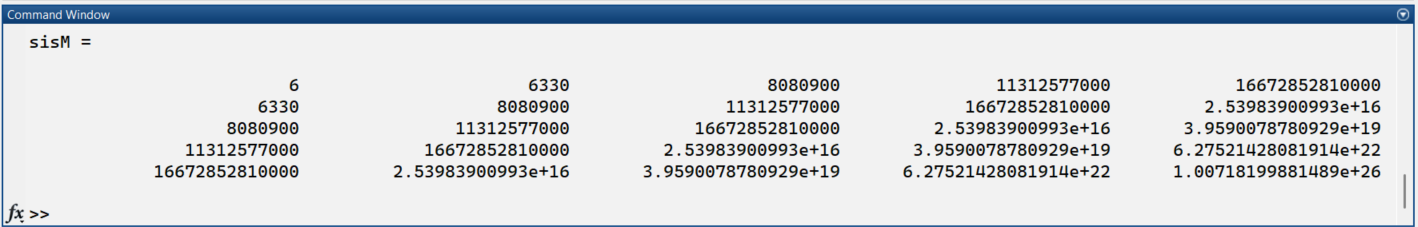
\includegraphics[width=6in]{sisM.png}
\caption{Matriz obtenida con el método}
\label{figure:sisM}
\end{figure}

Con la matriz creado es momento de pasar a resolver el sistema para obtener los coeficientes del polinomio y posteriormente, la respuesta al problema.
\begin{figure}[H]
\begin{tcolorbox}[title=Ejemplo 2: Implementación en MATLAB]
\begin{verbatim}
%Resolver el sistema de ecuaciones
detM=det(sisM); % lo guardamos para no requerir calcularlo siempre
for i=1:k
   newMatrix = sisM;
   newMatrix(:,i) = resM;
   coeficientes(i) = det(newMatrix)/detM;
end
% Generando el polinomio
pol = coeficientes(1);
for i=2:k
    pol = pol + coeficientes(i)*x^(i-1);
end
estimacion = double(subs(pol,xEvaluar)); %% Respuesta
\end{verbatim}
\end{tcolorbox}
\end{figure}
\begin{figure}[H]
\centering
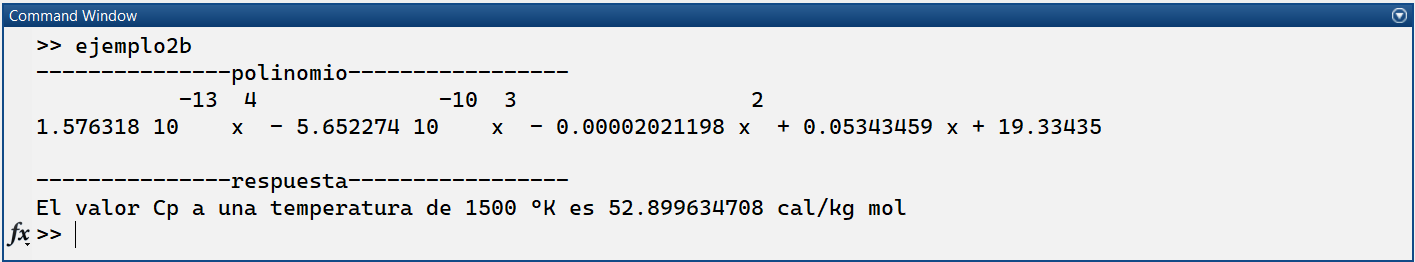
\includegraphics[width=6in]{ej2ans.png}
\label{figure:ej2ans}
\end{figure}

\subsubsection*{\textcolor{Mahogany}{Problema asignado usando el método de ajuste de polinomios de grado $n=3$}}
\begin{center}
\textit{\textbf{Problema 5:} En un experimento se desea encontrar una expresión matemática que relacione la concentración de un medicamento en el organismo en función del tiempo. Se dispone de los siguientes datos experimentales:}\linebreak\par
	\begin{tabular}{c|cccccccc}
	\hline 
	Tiempo (min) & 0 & 4 & 10 & 19 & 35 & 55 & 75 & 85 \\ 
	\hline 
	Concentración & 100 & 69.62 & 32.32 & 24.1 & 12.54 & 5.63 & 3.74 & 2.99 \\ 
	\hline 
	\end{tabular} \linebreak\par
	\textit{Ajuste un polinomio de mínimos cuadrados de tercer grado. Represente gráficamente la función de aproximación junto con los datos y estime el valor de la concentración al cabo de 50 y 100 minutos.}
\end{center}
Para resolver este problema, haremos uso del algoritmo presentado en el ejemplo anterior, pero haciendo uso de los datos de este problema.
\begin{figure}[H]
\begin{tcolorbox}[title = Problema 5: Valores y sumas iniciales en el algoritmo]
\begin{verbatim}
% Valores del tiempo
X = [0 4 10 19 35 55 75 85]; 
% Concentración del medicamento
Y = [100 69.62 32.32 24.1 12.54 5.63 3.74 2.99];
xEvaluar1 = 50; % En un tiempo 50 (interpolación)
xEvaluar2 = 100; % En un tiempo 100 (extrapolación)

% Se ocupará un polinomio de grado 3 como se indica
n = 3;
% Guardar el valor de la sumatoria de Y
sumY = sum(Y);
\end{verbatim}
\end{tcolorbox}
\end{figure}
A continuación, llenaremos en un vector las sumas de todos los valores de $X$ elevados a sus potencias desde 1 hasta $2n$. Posteriormente, crearemos un vector que almacene los valores de la submatriz de resultrados.
\begin{figure}[H]
\begin{tcolorbox}[title = Problema 5: Vector de sumas y vector de resultados]
\begin{verbatim}
%Guardar en un vector las sumas de todos los valores de X elevadas a sus
%potencias desde 1 hasta 2n 
for i=1:2*n
    sum = 0;
   for j=1:length(X)
       sum = sum + (X(j))^i;
   end
   sumXs(i) = sum;
end
% Creando un vector que almacene los resultados de la matriz
for i=1: n+1
    if i == 1
        resM(i) = sumY; 
    else
        sumatoria = 0;
        for j=1:length(X)
             sumatoria = sumatoria + Y(j)*X(j)^(i-1);
        end
        resM(i) = sumatoria;
    end
end
\end{verbatim}
\end{tcolorbox}
\end{figure}

Ahora podemos pasar a la creación de la matriz del sistema de ecuaciones con las sumas y resultados obtenidos. Posteriormente, con la matriz resuelta podremos armar el polinomio de grado 4 que usaremos para aproximar los valores de la función.
%% MATRIZ
\begin{figure}[H]
\begin{tcolorbox}[title = Problema 5: Creación de la matriz del sistema de ecuaciones]
\begin{verbatim}
%Creando la matriz del sistema de ecuaciones
k = length(resM);
sisM = zeros(k);
%Llenando la primera fila
for j=1:k
    if j == 1
        sisM(j,j) = length(X);
    else
        sisM(1,j) = sumXs(j-1);
    end
end
%Llenando el resto de filas
for i=2:k
   for j=1:k
       if(i == 2)
           sisM(i,j) = sumXs(j);
       else
           sisM(i,j) = sumXs(i+j-2);
       end
   end
end
sisM(k,k) = sumXs(2*n);
\end{verbatim}
\end{tcolorbox}
\end{figure}
%%POLINOMIO
\begin{figure}[H]
\begin{tcolorbox}[title = Problema 5: Resolución de la matriz del sistema y generación del polinomio]
\begin{verbatim}
%Resolver el sistema de ecuaciones
detM=det(sisM);
for i=1:k
   newMatrix = sisM;
   newMatrix(:,i) = resM;
   coeficientes(i) = det(newMatrix)/detM;
end

% Generando el polinomio
pol = coeficientes(1);
for i=2:k
    pol = pol + coeficientes(i)*x^(i-1);
end
estimacion1 = double(subs(pol,xEvaluar1));
estimacion2 = double(subs(pol,xEvaluar2));
\end{verbatim}
\end{tcolorbox}
\end{figure}

A continuación mostraremos la ejecución final del algoritmo, junto con los valores de la matriz obtenida en \textit{MATLAB}, los resultados de la evaluación  y el polinomio obtenido. \footnote{Es necesario hacer énfasis al lector en este punto que \textit{MATLAB} no es un software sin problemas, y los determinantes de matrices pueden ser erróneas debido al algoritmo usado, el cual es vulnerable a errores de punto flotante.}

\begin{figure}[H]
\centering
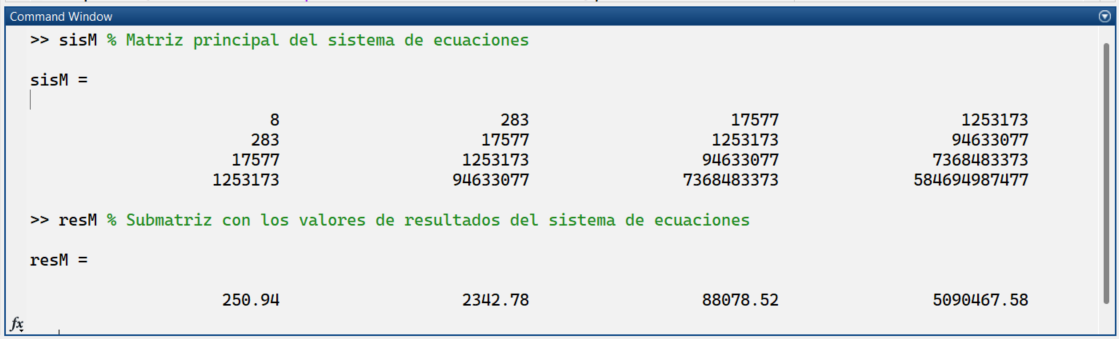
\includegraphics[width=5in]{mtz5.png}
\caption{Matriz resultante de $4\times 4$ con los valores del sistema de ecuaciones del método. Abajo, la submatriz con los resultados del sistema de ecuaciones obtenido}
\label{figure:mtz5}
\end{figure}

\begin{figure}[H]
\centering
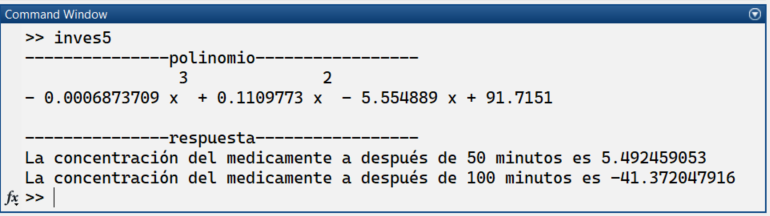
\includegraphics[width=5in]{res5.png}
\caption{Polinomio resultante con los coeficientes siendo las respuestas de la matriz del sistema de ecuaciones. Abajo, los resultados obtenidos de las evaluaciones, dando así, los valores de las estimaciones finales}
\label{figure:res5}
\end{figure}
%Grafica
\begin{figure}[H]
\centering
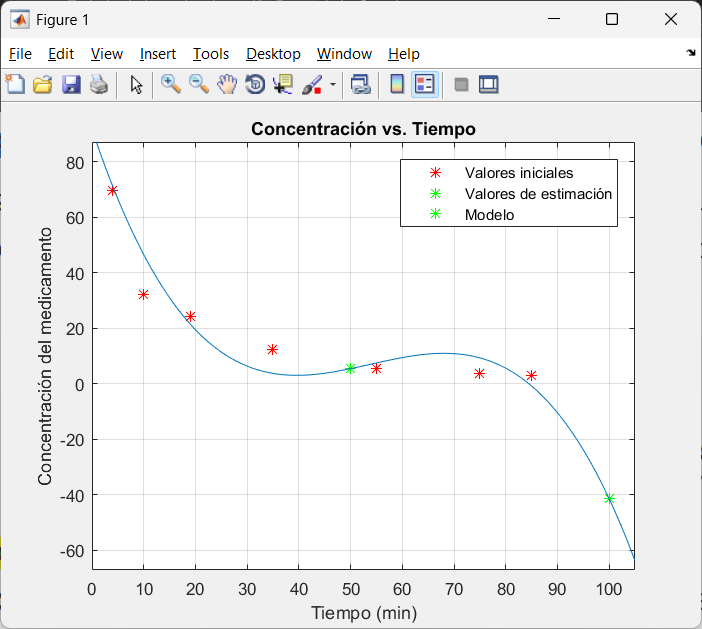
\includegraphics[width=3in]{graf5.png}
\caption{Gráfica del modelo polinomial encontrado, mostrando los puntos iniciales sobrepuestos, junto con los valores de aproximación}
\label{figure:graf5.png}
\end{figure}


%+++++++++++++++++++++++
% BIBLIOGRAFIA
% +++++++++++++++++++++++
\bibliographystyle{IEEEtran}
\bibliography{bibi}

\end{document}